\documentclass[a4paper]{scrreprt}
\usepackage[utf8]{inputenc}  \usepackage[T1]{fontenc}
\usepackage{lmodern}           \usepackage[ngerman]{babel}
\usepackage{fullpage}
\usepackage{graphicx}
\usepackage{color}
%\usepackage{geometry}
\DeclareUnicodeCharacter{B0}{$^{\circ}$}
%\geometry{a4paper,left=3cm,right=3cm, top=3cm, bottom=3cm}

\parindent0em
\parskip5pt

\usepackage[hyphens]{url}
\usepackage[pdfborder={0 0 0},breaklinks,colorlinks,urlcolor=blue,linkcolor=blue,citecolor=black]{hyperref}
%\urlstyle{rm}

\begin{document}

\title{Über Leben in Berkeley}

%\maketitle
\begin{center}

\vspace{0.4\textwidth}
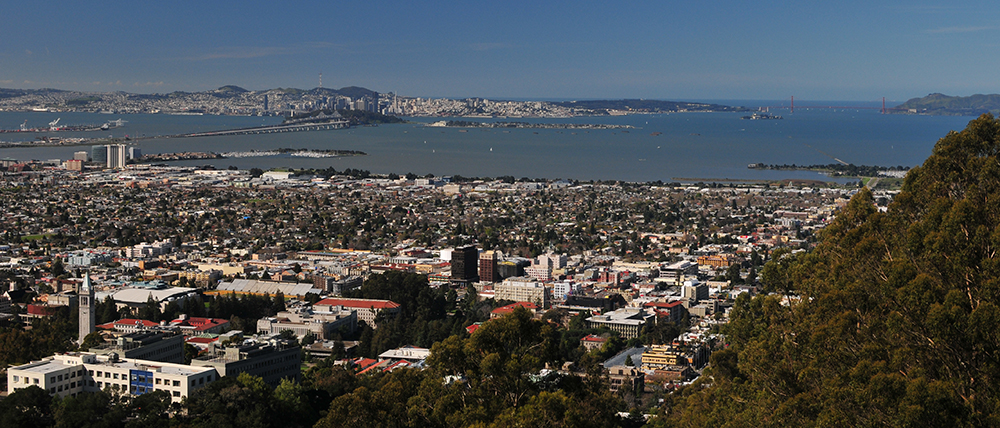
\includegraphics[width=0.8\textwidth]{img/berkeley_cropped.jpg}

\vspace{0.1\textwidth}
\Huge{\textbf{Über Leben in Berkeley}}
\end{center}

\newpage

\section*{Willkommen in Berkeley!}

Der Name Berkeley ist wohl in der ganzen Welt bekannt, und das liegt vor allem an der Universität, ohne welche die Stadt mit ca. 100.000 Einwohnern wohl nur einer unter vielen suburbs von The City (San Francisco) wäre. So muss man schon beim Parken auf dem Campus aufpassen, da einige Parkplätze für NL (=Nobel Laureate) reserviert sind.

Im Folgenden berichten wir (die aktuellen und ehemaligen DAAD-ICSI-Stipendiaten) von unserem Berkeley-Aufenthalt - wir haben hier unsere Erfahrungen zu Vorbereitung, den ersten Schritten in Berkeley und all den vielen Dingen, die man sehen, schmecken, besuchen und erleben sollte, gesammelt als Hinweise für die kommenden Stipendiatsgenerationen. Eingeflossen sind dabei auch die verschiedenen Berichte, die im Laufe der Jahre beim ICSI eingereicht wurden und wir hoffen das dieser Bericht weiterhin stetig aktualisiert wird.

Für den schnellen Einstieg haben wir versucht, den Bericht zeitlich zu ordnen: Der erste Teil (Visum, Reiseplanung, ...) sollte möglichst direkt angegangen werden. Die nachfolgenden Teile über das Einleben in Berkeley können dann aber auch erst auf dem Flug gelesen werden und gerade die abschließenden einzelnen kurzen Berichte über all das, was man in Berkeley und größerer Umgebung machen kann, sollen eher als Nachschlageverzeichnis dienen.

%Jetzt kann die Vorfreude auf Berkeley beginnen!

\tableofcontents
 
\chapter{Vorbereitung: Visum, Anreise, ...}

\section{Visum}

Um in die USA einreisen zu können, benötigt man als ICSI-Stipendiat ein J1-Visum und mitreisende Angehörige ein J2-Visum. Die Beantragung des Visums und der dafür notwendigen Unterlagen dauert seine Zeit. Daher sollte dies gleich nach Erhalt der DAAD-Unterlagen angestoßen werden. Was braucht man alles, um ein Visum zu bekommen?

\begin{itemize}

  \item Einen deutschen Pass; wenn nicht vorhanden muss dieser beantragt werden und bei der Beantragung sollte man das Ablaufdatum erfragen, da dies fürs Visum benötigt wird. Ein deutscher Reisepass muss bis Ende des Visums gültig sein. Kinder (auch Babys) benötigen einen Kinderreisepass, ein Eintrag im Pass der Eltern oder der alte (grüne) Kinderausweis genügt nicht.

	\item Ein DS-2019; hierzu muss der E-Mail-Fragebogen des International Office der UC Berkeley zur Erstellung des DS-2019 ausgefüllt und abgeschickt werden. Man wird dafür vom International Office angeschrieben.
	
	\item Einen Interviewtermin bei der Botschaft, den man vereinbart, wenn man das DS-2019 zugeschickt bekommen hat. Die Visa-Unterlagen gemäß dem aktuellen Antragsverfahren - da das Antragsverfahren sich dauernd ändert, muss man die aktuell notwendigen Unterlagen für Visa auf der Website der deutschen US-Botschaft (\url{http://germany.usembassy.gov/}) einsehen.

\end{itemize}

Im folgenden noch einige Anmerkungen zu den einzelnen Unterlagen und deren Beantragung.

\begin{enumerate}
	\item \textbf{Das DS-2019:} Das DS-2019 bescheinigt einem vom Gastinstitut (dies ist offiziell die UCB), dass man als Stipendiat dort angenommen ist und dadurch für ein J-1 Visum infrage kommt. Zur Beantragung bekommt man auf Anfrage einen Fragebogen vom ICSI zugemailt, den man nur ausgefüllt zurückschicken muss (das ICSI übernimmt die Kommunikation mit dem International Office). Benötigt wird hier das Ablaufdatum des Passes. Wenn ein neuer Pass für den ICSI-Aufenthalt beantragt wird, kann das Ablaufdatum direkt bei der Beantragung erfragt werden. Einige Wochen später bekommt man das DS-2019 vom International Office der UC Berkeley ausgestellt und per Kurier zugestellt.
	
	Wir empfehlen, den Fragebogen direkt auszufüllen. Während das DS-2019 und ggf. der Pass erstellt werden (was 1-2 Monate dauert), können die restlichen Visumsunterlagen zusammengestellt werden. Die aktuellen Formulare sind auf der Website der US-Botschaft erhältlich. Mit Pass und DS-2019 hat man die Daten, um ein weiteres Formular auf der Homepage der US-Botschaft zu erzeugen (DS-160), das man direkt ausdrucken kann. Die Daten dieses Formular werden wiederum benötigt, um einen Termin beim Konsulat zu beantragen. Bei der Ausstellung des DS-2019 wird vom ICSI die SEVIS (Student and Exchange Visitor Information System) Gebühr bezahlt. Hierfür erhält man vom ICSI den beim Visumsinter- view notwendigen Zahlungsbeleg zusammen mit dem DS-2019 zugeschickt.

	\item \textbf{Interview in einer US-Botschaft:} Um ein Visum zu bekommen, ist ein kurzes Interview in einer US-Botschaft notwendig. In Deutschland befinden sich diese in Frankfurt, Berlin und München. Der Termin für ein solches Interview kann telefonisch oder online (beides gebührenpflichtig) vereinbart werden. Vor Semesterbeginn in den USA (August, September) sind Termine oft knapp, weil die Botschaften dann viele Studentenvisa bearbeiten. Bei der Wahl der US-Botschaft sollte man darum nicht nur nach örtlicher Nähe, sondern vor allem nach der stark differierenden Wartezeit für Interviewter- mine vorgehen. Vorteil des derzeitigen Interview-Verfahrens ist, dass die Bearbeitung in der Regel schnell geht und man den Pass mit dem Visum etwa drei Tage nach dem Interview im Briefkasten hat (in dieser Zeit hat man keinen Pass!). Das Visum sollte man unbedingt auf Korrektheit überprüfen.
	
	Generell gilt: Das DS-2019-Formular ist mindestens genauso wichtig wie der Pass. Dieses Formular sollte bei der
Einreise auf jeden Fall im Handgepäck sein.
	
	Das DS-2019 muss nach der Ankunft in Berkeley im International House unterschrieben werden. Hierfür gibt es feste Termine, die man am ersten Tag am ICSI mitgeteilt bekommt oder online nachlesen kann.

	\item \textbf{Gebühren:} Bei der Onlineanmeldung zum Interviewtermin und Zusammenstellung der Visumsunterlagen muss eine Gebühr entrichtet werden (derzeit 10,- EUR). Dazu kommt eine Visumsantragsgebühr (99,56 EUR pro Person, auch für Kinder), die über die Kanzlei Roskos \& Meier bezahlt wird. Roskos \& Meier senden die Zahlungsbestätigung nach Gelderhalt an den Antragssteller.

	Familien und andere Gruppen von Antragstellern können eine Überweisung tätigen, es wird jedoch für jeden eine eigene Zahlungsbestätigung ausgestellt, die dann mit dem individuellen Antrag beim Interviewtermin eingereicht wird.
	
	Das Verfahren über Roskos \& Meier dauert ein paar Tage und muss beim Interviewtermin abgeschlossen sein. Wenn die Zeit knapp ist (zum Beispiel, weil einem in letzter Minute auffällt, dass man diese Gebühr noch zahlen muss), können auch Einzelpersonen das Geld direkt überweisen und dann den Beleg beim Interview vorlegen. Dies ist zwar offiziell die Regelung für Notfälle, ist allerdings im Sommer 2010 ohne weitere Nachfrage akzep- tiert worden.
	
\end{enumerate}

\section{Anreise}

Kalifornien hat eine Menge zu bieten und der Spätsommer ist eine perfekte Reisezeit. Daher bietet es sich an, die Zeit vor Stipendienantritt schon für eine kleine Rundreise zu nutzen (siehe Reisetipps hinten). Der nächstgrößere Flughafen von Berkeley aus ist San Francisco Airport (SFO). Alternativ kann man auch nach Oakland (OAK) fliegen, allerdings gibt es nach dort keine Direktflüge von Deutschland aus. Die preislich günstigste Airline (und damit zusammenhängend auch Reiseroute) wechselt ständig. Daher ist es am einfachsten hier eine Reiseplattform zu nutzen. Mit www.expedia.com haben wir gute Erfahrungen gemacht (für inner-amerikanische Flüge gibt es noch spezielle Plattformen wie  www.kayak.com). Empfehlenswert ist auch  \url{www.swoodoo.com}, eine Meta-Suchmaschine in der expedia, opodo u.a. durchsucht werden. Preise sind saisonabhängig, liegen aber für Hin- und Rückflug im Bereich zwischen 500 und 900 Euro. Wer nur einen Hinflug buchen will oder noch kein Rückflugdatum hat (bzw. dieses ist erst ein Jahr später und dann noch nicht direkt buchbar, da bei den meisten internationalen Airlines nur 11 Monate im voraus gebucht werden kann), kann auch mit Air Berlin fliegen. Im Sommerflugplan (bis Ende September) bietet Air Berlin die Strecke Düsseldorf-San Francisco als Direktflug an. Sinnvoller ist es aber oft den Rückflug nachträglich gegen Gebühr umzubuchen. Zum Beispiel kostet diese Umbuchung bei British Airways \$150. 

Bei der Auswahl des Tickets lohnt es sich darauf zu achten, wie viel Gepäck man mitnehmen darf. Dieses ist seit kurzem bei nahezu allen Airlines auf ein Gepäckstück zu 23 kg je Person beschränkt, ein weiteres Gepäckstück kann für ca. 50 EUR hinzugekauft werden. Bei manchen Fluggesellschaften ist die Mitnahme eines Sportgerätes (auch Fahrrad) kostenlos möglich.

Insbesondere wenn man mit Kindern reist, sollte man bei der Auswahl der Airline kritischer sein und auf den Service achten. Abzuraten ist hier insbesondere von American Airlines, da es hier z.B. für Kleinkinder unter 2 Jahren (also ohne eigenen Sitzplatz) nichts zu essen gibt und das Kinderbett aus einer Pappschachtel besteht.

Bei der Buchung eines Fluges haben Umstiege in Amerika den Nachteil, dass man am ersten amerikanischen Flughafen alle Einreiseformalitäten erledigen muss. Dabei muss auch das Gepäck ausgecheckt und erneut wieder aufgegeben werden; dies kann zu Problemen mit dem Anschlussflug führen. Vom Flughafen (SFO oder OAK) nach Berkeley kommt man mit der BART (60 bzw. 45 Minuten, günstig, unproblematisch und zu empfehlen), Taxi bzw. Bayporter (30-40\$) oder einem ab Flughafen gemieteten Mietwagen.
 
\section{Wohnen in Berkeley}

Das Mietpreisniveau in Berkeley ist höher als in deutschen
Universitätsstädten. Nahe beim ICSI und damit relativ zentral muss man
damit rechnen, dass man für ein WG-Zimmer um 600\$ zahlt und für ein
kleines Apartment ab 1100\$ aufwärts -- Blick auf die Bay oder Golden
Gate Bridge kostet extra. Das ICSI hilft gerne und kompetent bei der
Vermittlung, wenn man das dafür zugemailte Formular an sie frühzeitig
zurücksendet. Man bekommt konkrete Wohnungsangebote und die
Kontaktdaten der jeweiligen Vermieter per E-Mail übermittelt. Das
Angebot beinhaltet eine Beschreibung der Wohnung und Bilder der
Zimmer. Die ICSI-Angebote befinden sich meist in nicht allzu großer
Entfernung zum Institut und entsprechen eher einem etwas gehobeneren
Wohnstandard, der mit Deutschland vergleichbar ist. Hat man kein Auto,
sollte man versuchen, in Lauf-/Fahrradfahrentfernung vom 
ICSI zu wohnen oder in der Nähe einer BART-Station (der
U-Bahn). Sollte man sich für den (schönen) Osten Berkeleys
entscheiden, dann sollte man berücksichtigen, dass es aufgrund des
bergigen Terrains teilweise mühsam, aber mit dem Fahrrad machbar
ist. Wenn man allerdings auch mal eine Gallone Milch kaufen möchte,
empfiehlt sich dann ein Auto, um die größeren Potentialunterschiede zu
überwinden. Eine Busanbindung ist teilweise gegeben, aber abends endet
der Service oft gegen 20 Uhr.

Die Orte Albany und El Cerrito nördlich von Berkeley bieten sicheres
und familienfreundliches Wohnen zu etwas moderateren Preisen als
direkt in Berkeley. Was den Weg zum ICSI angeht, gibt es einen
verkehrsberuhigten Fahrradweg nach Berkeley (den Ohlone Greenway) oder
die BART. Pendeln mit dem Fahrrad aus El Cerrito dauert etwa 30
Minuten pro Strecke, aus Albany etwa 20 Minuten.

Neben der ICSI-Vermittlung kann man sich auch selbst nach einer
Wohnung umsehen, wodurch man eine größere Auswahl hat und ein
preislich günstigeres Angebot finden kann. Die unmöblierten Angebote
in Berkeley sind oft durchaus 200\$ günstiger als die möblierten, die
vom ICSI angeboten werden. Dadurch kann man Geld sparen, wenn man sich
die Grundausstattung an Möbeln selbst bei Ikea oder über Craigslist
zusammenstellt. Möbel und Hausrat sind günstiger als in
Deutschland. Mietverträge für Wohnraum werden sowohl auf Monatsbasis
als auch auf Ein-Jahres- Basis abgeschlossen und die Bereitschaft,
gleich einen Ein-Jahres-Vertrag abzuschließen, kann ein Argument sein,
um eine Mietreduzierung auszuhandeln. Es gibt sowohl die all-inclusive
"`Warmmiete"' als auch Wohnungen, bei denen der Mieter Wasser, Strom
und Heizung selbst bezahlen muss. Generell sollte man sich darauf
einstellen, dass die Qualität der Wohnungen in der Regel nicht mit
deutschem Standard vergleichbar ist. So sind Wände oft hellhörig und
schlecht wärmeisoliert.

Craigslist ist auch eine gute Anlaufstelle für die Wohnungssuche im
Internet, in der man kostenfrei annoncieren kann (Warnung: Hier gibt
es auch betrügerische Angebote. Daher nie Geld aus dem Ausland
überweisen und Wohnungen vor dem Unterschreiben des Mietvertrages
besichtigen.).

Da mit Wechsel des DAAD-Stipendiatenjahrgangs Anfang September gleich
mehrere Wohnungen oder Zimmer frei werden, kann man auch direkt
Kontakt aufnehmen. Neben Wohnung lassen die abreisenden Stipendiaten
zudem einiges an Hausrat, Fahrrädern, Autos, \dots\ zurück und hier kann
man kostengünstig solche Dinge übernehmen.

Darüber hinaus beschäftigt sich die Postdoc-Net-Mailingliste
hauptsächlich mit Wohnungsauflösungen, Mietgesuchen und -angeboten
oder dem Gebrauchtwagenverkauf. Wir empfehlen sich gleich unter
\url{https://calmail.berkeley.edu/manage/list/listinfo/postdocnet@lists.berkeley.edu}
einzuschreiben.

Wer sich zuerst einmal in Berkeley umschauen möchte, um dann in Ruhe
eine Wohnung zu suchen, kann das Angebot von
\url{https://www.airbnb.com} nutzen. Über diese Webseite werden 
Zwischenmieten für Wohnungen und WG-Zimmer vermittelt. 

\section{Krankenversicherung und Ärzte}

Als DAAD-Stipendiat gilt man als Visiting Scholar der UCB und muss krankenversichert sein (Bedingungen für die Krankenversicherung gibt es beim International Office:  \url{http://internationaloffice.berkeley.edu/j\_insurance}). Der DAAD bietet eine Gruppenauslandskrankenversicherung (Continentale) an, mit der man gut fährt. Alternativen sind die Mawista (Würzburger), Victoria, DKV, UKV, oder ACE, die deutlich günstiger als die Gruppenauslandskrankenversicherung des DAAD sind (bei der Mawista gelten Postdocs noch als Studenten). Die Bedingungen sind bei allen ähnlich und schließen Kosten aus bestimmten Anlässen (z.B. vor Versicherungsantritt, Vorerkrankungen, Vorsorgeuntersuchungen) aus. Einige deutsche Anbieter (u.a. die genannte Mawista) kooperieren mit US-amerikanischen Versicherungen, so dass man bei einer Behandlung nicht in Vorkasse treten muss, sondern einfach die Versichertenkarte vorzeigt. Der behandelnde Arzt kann dann über das lokale System abrechnen, und man selbst muss die Rechnungen nicht mehr bei der deutschen Versicherung einreichen. Die DAAD-Versicherung kooperiert mit der Firma Global Medical Management (GMM) in Florida. Man kann von dieser Firma einen Versicherungsausweis erhalten (Online zum selbst ausdrucken) und theoretisch kann der Arzt die Behandlungskosten dann direkt mit GMM abrechnen. Auf der Homepage der Continentale/GMM gibt es eine Liste von Ärzten, bei denen man sich behandeln lassen kann ohne Vorkasse zu leisten.
Wenn man sich für einen Arzt entscheidet, der nicht auf der GMM-Website gelistet ist, sollte man sich vorher erkundigen, ob der betreffende Arzt trotzdem zu einer Behandlung bereit ist.

Bei der Auswahl der Krankenversicherung sollte man berücksichtigen, in welchem Umfang die Auslandskrankenversicherung Behandlungen in Deutschland abdeckt (z.B. Familienurlaub oder Bewerbungsreise), da die Sozialversicherung zu Hause normalerweise für die Dauer des Auslandsaufenthalts ruht. Hier ist die Versicherung des DAAD sehr flexibel. Wenn Vorerkrankungen eine Rolle spielen, sollte man sich den ICSI-Bericht von Marek Musial besorgen.

In bestimmten Fällen ist eine US-amerikanische Krankenversicherung besser oder sogar unerlässlich (z.B. Bestehen einer Schwangerschaft vor Versicherungsbeginn). In diesem Fall reist man mit einer einfachen Reisekrankenversicherung ein und schliesst dann vor Ort eine Versicherung ab, z.B. beim University Health Service (UHS) oder bei Kaiser Permanente, der Krankenversicherung des ICSI, welche die Inanspruchnahme von Gesundheitsleistungen teilweise wesentlich vereinfacht.

Es gibt eine Reihe von Arztpraxen in Berkeley und jeder kann sich einen Arzt seines Vertrauens suchen. Falls man sich darüber noch keine Gedanken gemacht hat und schnell einen Arzt braucht, ist sicher das University Health Services / Tang Center eine gute Anlaufstelle. Hier finden sich Ärzte aller Fachrichtungen unter einem Dach, außerdem sind eine Apotheke und ein Labor angeschlossen. Dieses Ärztehaus ist in erster Linie für Studenten und Mitarbeiter der Uni gedacht. ICSI-Stipendiaten und deren Ehepartner können sich dort behandeln lassen, nicht jedoch deren Kinder.
Eine Kinderärztin mit recht gutem Ruf ist Karin Schiffman in 2500 Milvia Street, Raum 102 (Tel.: (510) 845-0300). Verschreibungspflichtige Marken-Medikamente sind in den USA sehr teuer. Man kann oft deutlich sparen, wenn man Generika, z.B. aus dem Internet bestellt.
 
\chapter{Erste Schritte in Berkeley}
%\chapter{Erste Schritte: How to survive in Berkeley}

\section{Von Ort zu Ort mit Rad, Bus, BART und zu Fuß}

Fahrräder sind ein gutes Fortbewegungsmittel in Berkeley. Es gibt
viele Radwege und extra Radstraßen. In der BART und im Bus kann man
Räder ohne Aufpreis mitnehmen. Man sollte berücksichtigen, dass die
Höhenprofile sehr unterschiedlich sind. Es kann sich also lohnen
Umwege zu fahren.

Die Preise für Fahrräder sind vergleichbar mit deutschen
Preisen. Einfache gebrauchte Fahrräder in gutem Zustand gibt es
zwischen 150\$ bis 200\$. Günstige neue Fahrräder findet man ab etwa
300\$. Dazu kommen unbedingt noch Licht und ein Schloss, da
Fahrraddiebstahl und auch Reifen- und Lichtdiebstahl in Berkeley
leider verbreitet sind. Deshalb sollte man ein langes Kabel und ein
Bügelschloss kaufen, um Vorder- und Hinterräder zu sichern. Gute
Adressen, um an ein Rad zu kommen, sind:

\begin{itemize}
\item abreisende Postdocs: ehemalige ICSI-Stipendiaten oder Angebote
  auf der Postdoc-Net Mailingliste
\item craigslist
% \item Karim Cycle, 2800 Telegraph Ave, hat eine große Auswahl an
%   gebrauchten Rädern, die zum Teil auch brauchbar sind.
\item Missing Link, eine Bicycle-Coop mit Werkstatt zum
  Selbstreparieren an der Shattuck Ave, Ecke University. Hier findet man
  aber nur selten gebrauchte Fahrräder.
\item Mike's Bikes, 2161 University Ave. Hier gibt es neue Fahrräder
  teilweise schon ab 200\$. Mittwochnachmittags kann man hier kostenlos
  auf Werkzeug und fachkundigen Rat zurückgreifen, wenn man sein
  Fahrrad reparieren möchte.
\item Performance Bicycles, 1824 University Ave. Hier gibt es ebenfalls
  günstige neue Fahrräder und günstiges Zubehör wie Helme und Pumpen. 
% \item Ashby Flea Market. Günstige Gebrauchträder und
%   Ersatzteile. Wenn das eigene Rad mal gestohlen wurde, ist die Chance
%   groß, dass man es hier zurückkaufen kann.
\item Watersite Workshop, 84 Bolivar Drive. Ist sehr zu
  empfehlen, hat allerdings nur Freitag, Samstag und Sonntag von 12
  bis 18 Uhr geöffnet. Hier bekommt man gebrauchte Räder, aber auch Ersatzteile
  zum kleinen Preis. Sie verfügen über eine Fahrradwerkstatt, in der
  man sein Fahrrad selbst reparieren kann. Aber keine Angst, die Mitarbeiter
  stehen mit Rat und Tat zur Seite. Neben der Fahrradwerkstatt gibt es das
  Waterside Café mit bequemen Holzstühlen direkt am Wasser. 
\end{itemize}

Zu empfehlen sind Fahrrad- und Wanderkarten von Rufus Guides, die man
in jedem Buchladen bekommt. Auf den Karten von Berkeley und San
Francisco sind mit unterschiedlichen Farben die Steigungen
markiert. Diese kann man dann versuchen zu umfahren, obwohl es sich
auch lohnt die eine oder andere Steigung mit dem entsprechenden
Ausblick und der Abfahrt zu nehmen. 

Für Tripplanner und Maps der lokal-regionalen Bussysteme empfiehlt
sich \url{http://511.org} oder man nutzt
\url{http://maps.google.com}. Mit den Bussen
(\url{http://www.actransit.org/}) lassen sich die meisten Teile
Berkeleys erreichen, es gibt aber auch Verbindungen nach Oakland und
nach San Francisco. Eine Einzelfahrt kostet 2\$ -- das Geld muss man
passend haben, es wird nicht gewechselt. Alternativ kann man sich eine
Clipper Card holen, die gibt es umsonst und kann für alle öffentlichen
Verkehrsmittel der Bay Area eingesetzt werden. Aufgeladen werden kann
sie an S- und U-Bahnstationen und bei Walgreens
(Drogeriemarkt). Einige der Buslinien enden werktags bereits gegen 20
Uhr, am Wochenende sogar schon gegen 18 Uhr. 

Neben dem Bussystem gibt es in der Bay Area das S-Bahn-System BART
(Bay Area Rapid Transit). Die Tickets erhält man in den einzelnen
Stationen. Eine kurze, einfache Fahrt mit der BART ist (bei bis zu 4-5
Stationen) mit 1,75\$ nicht nur preiswerter, sondern auch
wesentlicher schneller. Aufgrund des dichten (7 1/2 Minuten werktags,
15 Minuten abends/am Wochenende) und längeren (bis 24 Uhr) Taktes ist
die BART-Fahrt der Busfahrt vorzuziehen. Fahrt von Berkeley nach San
Francisco kostet momentan ca. 4\$. San Francisco besitzt ein eigenes
S-Bahn und Straßenbahnnetz, die MUNI (San Francisco Municipal
Railway). Um mit der BART von San Francisco (bzw. dem Flughafen) nach
Berkeley zu gelangen, muss man entweder die BART nach Richmond (fährt
direkt nach Berkeley) oder nach Pittsburg/Bay Point nehmen. Bei
letzterer gibt es eine bequeme und zeitlich abgestimmte
Umsteigemöglichkeit an 19th Street Oakland (Northbound).

Auch zu Fuß kann man gut in Berkeley und Umgebung
unterwegs sein. Berkeley ist eine grüne Stadt, sogar in Downtown, und
es macht großen Spaß die Stadt durch  
Spaziergänge zu erkunden. Es gibt viele kleine Parks und
zwischendurch steht immer mal wieder ein alter großer Baum. Wie
zum Beispiel ein Redwood oder ein Eukalyptusbaum und auch viele
riesige Kakteen. % Wenn man sich dann noch vorstellt, dass hier 
% einmal Indianer gelebt haben, dann finde ich das schon sehr
% beeindruckend. 
Besonders an Berkeley ist, dass viele kleine Parks und Wohngebiete
durch Fußwege und Treppen verbunden sind. Kartenmaterial und
Informationen hierzu findet man in ``Berkeley's Pathway'' und dem
Buch ``Secret Strairs East Bay''. Auch in den Karten von Rufes Guides
sind Treppen und Wege eingezeichnet. Hat man diese erklommen, bietet
sich ein traumhafter Blick auf die Bay und die Golden Gate
Bridge.

\section{Auto mieten, kaufen, versichern}

In Berkeley und San Francisco kann man sich eigentlich sehr gut mit Rad, Bus und BART fortbewegen. Man sollte aber nicht vergessen, dass man in Kalifornien und damit auf einem besonders schönen Fleckchen Erde gelandet ist, das man auch ruhig erkunden darf. Wenn man dann auch noch ganz spontan zu einem Road Trip aufbrechen möchte, empfiehlt sich ein eigenes Auto.

Bei der Autoanschaffung muss man sich grundsätzlich entscheiden, ob man ein Auto vom Händler oder von einer Privatperson kauft. Wer es mit dem Autokauf nicht eilig hat, kann z.B. bei den verschiedenen Online-Plattformen auf gute Angebote warten, das Auto probefahren und durchchecken lassen und dann zuschlagen. Eine sehr gute Seite, um den Wert eines Wagens einzuschätzen, ist \url{http://www.kbb.com}. Hier lässt sich gut nachvollziehen, welche Unterschiede es zwischen Kauf von Privat und vom Händler gibt: Für einen 99er SUV mit 90.000 Meilen werden z.B. 6000\$ als Händlerverkaufspreis und 4300\$ als Preis für Privatverkauf vorgeschlagen. Andererseits geben Händler häufig Garantie, melden das Fahrzeug beim DMV an und können beim Abschluss einer Autoversicherung helfen. So oder so kommen zum Kaufpreis wie üblich ca. 10 \% Steuern dazu.

\begin{itemize}
	\item \textbf{Gebrauchtwagenkauf:} Gebrauchte Autos von Privat werden über die Craigslist oder über den Postdoc-E-Mail-Verteiler annonciert. Gerade über die Postdoc-Liste kommen häufig Angebote für Autos, die ein gutes Stück unter dem kbb.com-Preis liegen.

	In Berkeley gibt es u.a. den Zwischenhändler Buggybank, bei der Privatpersonen gegen Gebühr ihre Autos ausstellen können; man hat hier keine Garantie, dass die Wagen in Ordnung sind, aber man kann zu Geschäftszeiten Probefahrten machen und sich alles vorher im Internet anschauen (\url{http://www.buggybank.com}). Die Überprüfung durch einen Mechaniker ist hier dringend zu empfehlen und auch unkompliziert über Buggybank zu organisieren (80\$). Der Bericht des Mechanikers kann hier auch sinnvoll bei den Preisverhandlungen eingesetzt werden.
	
	Wichtiges Hilfsmittel für den Kauf ist carfax.com, eine Datenbank bei der man mittels der Fahrgestellnummer (Vehicle Identification Number - VIN) einen Teil der Vorgeschichte eines Fahrzeugs erfragen kann (5 Carfax re- ports kosten 45\$). So lassen sich die meisten faulen Eier (wie z.B. Unfallfahrzeuge) schon von vornherein aus- schließen. Wir haben bei unseren Recherchen durchaus auch ein paar solche Fälle erlebt, z.B. Auto, das auf Craigslist als "clean title" inseriert war, aber laut Carfax dann doch einen Unfall hatte. Vor dem Kauf eines Wa- gens sollte man einen Termin beim Automechaniker vereinbaren und den Wagen durchchecken lassen (50\$-100\$).

	Beim Privatkauf wird-um Steuern zu sparen-oft ein günstigerer "`offizieller"' Preis im Formular eingetragen und der Rest direkt bezahlt. Eine sehr detaillierte Beschreibung für den Kauf von Privat findet sich hier: \url{http://eagain.net/blog/2007/02/20/buy-a-car.html}. Hier ist auch das weitere Vorgehen beschrieben, wie z.B. die Anmeldung des Autos beim DMV, smog check usw..
	
	\item \textbf{Versicherung:} Die wichtigsten Komponenten des Versicherungsvertrags sind die Liability (Haftpflicht) und Comprehensive/Collision (die Schaden am eigenen Auto abdeckt). Die Haftpflicht umfasst Bodily Injury Liability, Property Damage Liability, und die Uninsured Motorist Bodily Injury (schützt den Fahrer, wenn bei einem Unfall der Verursacher unversichert war). Die Standardabdeckung gilt nur für die vom Staat vorgeschriebene Mindest- summe, z.B. Bodily Injury Liability 15/30, d. h. 15.000\$ pro Unfall und 30.000\$ insgesamt. Für deutsche Verhältnisse ist diese Deckung sehr gering und wir empfehlen, die Deckungssumme zu erhöhen, z.B. 100.000/300.000. Comprehensive/Collision kann ggf. weggelassen werden, wenn man sowieso ein sehr altes und billiges Auto gekauft hat.

	Wenn man in Deutschland schon einige Jahre unfallfrei fährt, kann man bei einigen Versicherungen einen Good Driver's Rebate bekommen, was die Kosten erheblich senkt. Einige Versicherungen wollen hierzu einen Nach- weis der deutschen Autoversicherung sehen, bei anderen kann man den Rabatt auch so bekommen (indem man angibt, man habe nie einen Unfall gemacht). In Frage kommen z.B. Progressive (bei der man auch übers Internet eine Policy abschließen kann), Mercury, das ADAC-Äquivalent AAA, oder auch Agenturen, die Policies verschiedener Anbieter verkaufen und dort etwas Günstiges anbieten können (z.B. Ozwald \& Speakar insurance services in Oakland). Eine Versicherung mit höheren Deckungssummen (allerdings ohne collision) kostete im März 2011 ca. 70-80\$ pro Monat. Damit ist zunächst der Halter der Fahrzeugs versichert und Familienmitglieder, die im selben Haus leben; wenn jemand anders den Wagen fährt, gelten die gesetzlichen Mindestsummen (15.000/30.000\$).
	
Kauft man bei einem Händler, kann dieser einem zunächst eine Versicherung (z.B. für den ersten Monat) verkaufen; dies ist unserer Erfahrung nach allerdings sehr teuer. Günstiger ist es, sich vorher eine Versicherung zu su- chen, telefonisch oder auf deren Webseite die Fahrzeugdaten durchzugeben, um sich dann die Versicherungsun- terlagen faxen zu lassen oder diese auszudrucken. Beim Händler bekommt man damit die restlichen Unterlagen und kann direkt losfahren.

	\item \textbf{Führerschein:} 
Wer in den USA Auto fahren möchte, benötigt einen kalifornischen Führerschein, da der deutsche für J1-Visums- Inhaber offiziell nur die ersten zehn Tage gültig ist. Daher sollte man-nachdem man seine SSN hat-die schrift- liche Führerscheinprüfung beim DMV (in El Cerrito oder in Oakland) machen (ein Termin ist eher nicht nötig, auf der Website kann man aber die aktuellen Wartezeiten recherchieren, damit man nicht zu lange anstehen muss).
Die Prüfung ist nicht teuer (32\$) und auch nicht schwer, wenn man sich vorbereitet (36 Multiple-Choice-Fragen, die auf dem California Driver Handbook basieren). Alle nötigen Infos gibt es im Internet (\url{http://dmv.ca.gov}). Mit der bestandenen schriftlichen Prüfung erhält man einen vorläufigen Führerschein, mit dem man dann die Praxis- prüfung beantragen kann. Wenn man einen deutschen Führerschein besitzt, kann man sich für die Prüfung ein Auto ausleihen. Wichtig ist dabei, dass man das Komplett-Versicherungspaket mitbucht, da dies beim DMV vor der Prüfung kontrolliert wird. Alternativ kann man den vorläufigen Führerschein auch regelmäßig kostenlos verlän- gern und muss so den (kostenlosen) Praxistest nicht mehr machen. Allerdings bekommt man dann auch keine California Driver's License, die als ID gerne gesehen wird (und im Portemonnaie sehr gut aussieht).

	J2-Reisende (also z.B. mitgereiste Ehepartner) müssen nicht auf ihre SSN warten und können gleich nach der Ein- reise den schriftlichen Test machen.

	\item \textbf{Parken:} Parken in Downtown-Berkeley und auch in San Francisco ist lächerlich schwierig. Die meisten Parkplätze für Nicht-Anwohner müssen nach 1-2 Std. mit Münzen gefüttert werden, wenn man den ganzen Tag in ICSI-Nähe parken müsste, ist man schnell über 15\$ los. Berkeley ist in verschiedene Parkzonen unterteilt, und man kann bei der Stadtverwaltung (im selben Gebäude wie das ICSI) ein Parking-Permit (ca. 35\$ für ein Jahr) bekommen, mit dem man dann in Wohnungsnähe parken kann. Dazu muss die vehicle registration card (auf dem die Wohnadres- se eingetragen ist) vorlegt werden. Wegen der schwierigen Parksituation eignet sich das Auto nicht zur täglichen Fahrt zur Arbeit (es sei denn, man braucht das Permit nicht fürs Parken bei der eigenen Wohnung und hat einen autolosen Kollegen, der beim ICSI wohnt; dann kann man seine Adresse beim DMV ändern, und so ein Permit in Arbeitsnähe bekommen).

	\item \textbf{Autovermietung:} Wer ein Auto für längere Zeit mieten will (beispielsweise für drei Wochen, wenn Besuch kommt), der sollte sich überlegen, den Wagen von Deutschland aus zu buchen (z. B. über  \url{http://www.billiger-mietwagen.de}). Dies ist oft billiger, wenn man alle Versicherungen einrechnet. Zu beachten ist, dass einem hier die Versicherungen für Miet- wagen immer gesondert verkauft werden. Oft ist ein Teil schon durch Premium-Kreditkarten abgedeckt. Preis und Ausstattung der Fahrzeuge kann erheblich variieren, genaues Hinschauen ist daher empfehlenswert.

	\item \textbf{Sonstiges:} Zur Überquerung der Brücken über die Bay muss man eine Maut zahlen. Wenn man länger mit demselben Wagen in der Bay Area unterwegs ist, lohnt es sich, einen FastTrak-Empfänger zu kaufen. Damit wird die Brückenque- rung elektronisch erfasst und die Gebühren direkt vom Konto abgehoben. Mit dem Gerät kann man auch die FastTrak-Spuren auf der Straße nutzen, auf denen man häufig schneller voran kommt. Den Empfänger gibt es z.B. bei Walgreens, er kostet 26\$, hat aber ein Maut-Guthaben von 30\$.

\end{itemize}

\section{Einkaufen}

Lebensmittel sind in Amerika deutlich teurer als in
Deutschland. Einkaufen kann man in Berkeley beim Supermarkt: Safeway
ist der klassische Supermarkt. Trader Joe's ist für ein etwas
günstigeres organic Angebot und günstigere EU-Produkte bekannt. Eine
recht große Mall findet man in Emeryville, auf der halben Strecke nach
San Francisco, wo sich auch ein IKEA befindet. 

In den Supermärkten (z.B. Safeway) gibt es Kundenkarten, über die man
Vergünstigungen bekommt. Die Karte kann man sich beim ersten Einkauf
direkt an der Kasse geben lassen und man spart so in der Regel etwa
10\%. Allgemein gibt es beim Einkauf immer und überall Aktionen
(Mengenrabatte, Sonderpreise, ...) durch die man weiter Geld sparen
kann. 

Großes Angebot und qualitativ gute Waren treffen sich im Berkeley Bowl
und im Monterey Market, allerdings auch zu höheren Preisen. In beiden
Märkten bekommt man Gemüse und Obst von den Bauern aus der
Umgebung. Es gibt ein großes Angebot an Bioprodukten. Gegenüber vom
Monterey Market gibt es das nette Café ``Esspresso Roma''

Die ausgewiesenen Preise sind Nettopreise, die Mehrwertsteuer muss man
also noch hinzurechnen. Als Faustregel gilt: Keine Steuer auf
Lebensmittel, auf alles andere sollte man 10\% aufschlagen.

Supermärkte haben in der Bay Area wenigstens bis 22 Uhr geöffnet. Auch
andere Läden, wie zum Beispiel Buchhandlungen, haben oft bis spät in
die Nacht geöffnet. Praktisch alle Geschäfte sind sonntags geöffnet.

Neben den Supermärkten gibt es in Berkeley verschiedene Wochenmärkte,
zum Beispiel wird direkt vor dem ICSI samstags ein kleiner Farmers'
Market abgehalten. Dort bekommt man Brot (u.a. von einem angeblich
Münchner Bäcker) und (Bio-)Gemüse. % Im Monterey-Market gibt es
% günstiges Obst und Gemüse von den Farmern der Umgebung.

Wer eine große Auswahl an Brot sucht, ist in der Bäckerei ACME Bread
(\url{http:/acmebread.com/}, 1601 San Pablo Avenue) gut aufgehoben. Zu
empfehlen ist das Edible Schoolyard Bread; ein Sauerteigbrot, das man
so in keinem anderen Geschäft in Berkeley bekommt. Außerdem gibt es
noch viele andere Brotsorten. Also keine Angst, auf
leckeres Brot muss nicht verzichtet werden! 

Günstig Kleidung einkaufen kann man gut in Outlet-Zentren, die aber
alle etwas weiter weg liegen
(\url{http://www.premiumoutlets.com}). Für ausgiebigere
Shopping-Vergnügen sollte man schon nach San Francisco fahren, viele
Shopping-Möglichkeiten gibt es zum Beispiel rund um die Powell
Station.

Kameras, Laptops oder ähnliches sind häufig am günstigsten über die
Bestellung im Internet. Pakete sollte man sich an die ICSI-Adresse
schicken lassen, da Lieferungen an die Wohnanschrift oft unangekündigt
und/oder unsanft vor der Haustür landen. Bei solchen Bestellungen kann
man unter Umständen die Steuer sparen, wenn die verschickende Firma
nicht in Kalifornien beheimatet ist.


\section{Konto und Kreditkarten}

Der einfachste Weg für den Zugriff auf das eigene Geld auf deutschen Konten ist durch direktes Zahlen mit Kreditkarten oder durch das Abheben von Geld an einem Geldautomaten (ATM). Beides ist häufig mit Gebühren verbunden. Eine der günstigsten Varianten bietet die DKB, bei der man mit einer VISA-Karte weltweit kostenlos an VISA-fähigen Geldautomaten Geld abheben kann. Allerdings entstehen bei vielen ATMs trotzdem Gebühren, die man sich aber bei der DKB (per email) wieder erstatten lassen kann. Die ATMs der Mechanics-Bank erheben bisher hierauf aber keine Gebühren.

Die Deutsche Bank hat ein Abkommen mit der Bank of America, so dass man als DB-Kunde an den BoA-Automaten gebührenfrei abheben kann. Kontoführungsgebühren entfallen, wenn man einen gewissen Mindestumsatz pro Monat hat oder aber ein Onlinekonto eröffnet (man kann sich dann allerdings nicht mehr direkt in der Bank beraten lassen).

Man sollte sich in jedem Fall ein amerikanisches Konto einrichten. Eine der ersten Aktivitäten in Berkeley sollte daher das Eröffnen eines Checking Accounts sein. Gute Erfahrungen wurden mit der Bank of America, der Wells Fargo-Bank, der Citi-Bank und der Mechanics-Bank gemacht. Alle vier haben Niederlassungen in der Nähe des ICSI und bieten kostenlose Online-Konten. Während bei der Bank of America nahezu alles online und am ATM erledigt werden kann, bietet Wells Fargo auch bei einem kostenlosen Konto einen hervorragenden persönlichen Service in den Filialen, erhebt dafür aber z.B. Gebühren für das Ansehen des Kontostandes am ATM.


Zur Kontoeröffnung sollte man den Reisepass mitnehmen und eine deutsche Kreditkarte, manchmal wird auch ein Adressnachweis verlangt. Wenn man seine Miete per Scheck bezahlen muss (das ist hier der gängige Weg) sollte man darauf achten, welche Kosten dies bei der entsprechenden Bank verursacht. Bei Chase und Mechanics bekommt man zur Kontoeröffnung einen Stapel Schecks geschenkt, bei der Bank of America muss man dafür zahlen. Bei Chase und der Bank of America können Schecks außerdem bequem und kostenfrei online in Auftrag gegeben werden, auch per Dauerauftrag. Die Bank stellt den Scheck dann aus und per Post an die angegebene Adresse zu.

Mit dem Konto bekommt man eine Debit-Karte, die wie eine Kreditkarte aussieht. Mit ihr kann man wie mit einer Kreditkarte bezahlen, nur dass das Geld sofort vom Konto abgebucht wird und kein Kreditrahmen besteht. In der Regel reicht das völlig aus. Allerdings gibt es überraschende Situationen, in denen man mit der Debitkarte nicht weiterkommt. Wenn die Karte als Sicherheit genutzt werden soll, wie beispielsweise beim Mieten eines Autos, wird die Debitkarte nicht akzeptiert. Für solche Situationen ist es gut, noch eine "`echte"' Kreditkarte (aus Deutschland oder meist gegen eine zusätzliche Gebühr für das amerikanische Konto) zu haben. Tipp: Bei manchen Kreditkarten ist auch gleich eine Mietwagenversicherung enthalten.

\paragraph{Bank Of America}  %von Daniel Goehring
Die Bank Of America besitzt eines der gr\"o\ss{}ten Filialnetze innerhalb der USA. Zur Er\"offnung eines Kontos ben\"otigt man lediglich einen Reisepass. Eine M\"oglichkeit, in den Genu\ss{} eines kostenlosen Girokontos (Creditaccount) mit vollem Schalter- und Onlineservice zu kommen besteht darin, auf dem Konto ein monatliches Durchschnittguthaben von 1500 Dollar zu besitzen (Stand: 02/2013). Aufpassen sollte man, dass man das Konto nicht \"uberzieht, denn hier werden schnell, wie bei anderen Banken auch, saftige Geb\"uhren f\"allig, d.h., 20 Dollar oder mehr. Einen Dispositionsrahmen gibt es leider nicht. F\"ur die Beantragung einer Kreditkarte ben\"otigt man eine Credit-History. Da diese zu Anfangs normalerweise nicht vorhanden ist, gibt es die M\"oglichkeit, eine Secure-Creditcard einzurichten, bei der man den Kreditrahmen selbst einzahlt. Diese Kostet pro Jahr 40 Dollar. Nach ca. 6 Monaten hat man damit eine ausreichende Credit-History aufgebaut und kann eine normale und kostenlose Kreditkarte beantragen. Auch hier ist es wichtig, angefallene Ausgaben immer zum Ende des Abrechnungszeitraumes auszugleichen, da sonst hohe Geb\"uhren anfallen.
Eine komfortable Option zur Bezahlung planbarer Ausgaben wie z.B. Miete besteht im kostenlosen Bill-Pay-Verfahren. Dabei kann man per Onlinebanking angeben, dass zu einem bestimmten Zeitpunkt in der Zukunft ein Check an den eigenen Vermieter / die Vermieterin per Post gesendet werden soll. Dieser kann nur von der Person, auf die der Check ausgestellt wurde, eingel\"ost werden. Dieser Service ist kostenlos und man spart sich den Kauf eines Checkbuches.

%%% Ende Teil Bank of America Daniel Goehring

\paragraph{Mechanics Bank}
Die Mechanics Bank (\url{https://www.mechanicsbank.com/}) ist der
Gegenentwurf zur Bank Of America. Sie ist eine lokal in der East Bay
angesiedelte Bank mit Filialen unter anderem in Berkeley und
Albany. Es gibt verschiedene Varianten ein kostenfreies Girokonto zu
bekommen, wobei die einfachste Möglichkeit ist, dass Guthaben auf dem
Konto nicht unter 1000\$ fallen zu lassen. Ein Girokonto, zu dem man
einen Stapel Schecks umsonst dazu bekommt, lässt sich vor Ort in der
Filiale in Berkeley ohne Social Security Number eröffnen. Die
zugehörige Debitkarte (oder zwei, falls man das Girokonto als Paar
führt) bekommt man nach ein paar Tagen per Post zugeschickt. Die
Mechanics Bank besitzt zwar selbst nur einige wenige Filialen und
Geldautomaten, erstattet aber Gebühren für die Nutzung von
Geldautomaten anderer Banken automatisch und wirbt mit ihrem
Telefonservice -- \emph{Talk to a real person}. Diesen kann man zum
Beispiel anrufen, wenn im Apple Store plötzlich die Debitkarte
streikt, man aber nicht ohne das schicke Notebook nach Hause gehen
möchte.

\paragraph{Geldtransfer aus Deutschland}

Die häufig günstigste Variante, Geld vom deutschen Konto auf das amerikanische Konto zu transferieren, ist, das Geld am ATM mit der Kreditkarte oder EC-Karte abzuheben und direkt am ATM auf das eigene Konto einzuzahlen (maximal 800\$ je Transaktion). Für den täglichen Bedarf ist dies vollkommen ausreichend. Für größere Ausgaben wie einen Autokauf sollte man hier aber rechtzeitig planen.

Ansonsten kann man Auslandsüberweisungen von Deutschland nach USA verwenden, muss aber dafür saftige Gebühren zahlen (ca. 15\$ pro eingehender Überweisung nehmen die amerikanischen Banken, von der deutschen Bank kommen in der Regel noch 2-4 EUR dazu). Bei größeren Beträge kann dies allerdings die günstigste Alternative sein.

\section{SSN Card: Social Security Number}

Die US-amerikanische Social Security Number (SSN) entspricht der deutschen Sozialversicherungsnummer, wird in den USA aber allgemein zur Bestimmung der Identität einer Person verwendet. Wenn man mit einem J1-Visum eingereist ist, benötigt man sie, wenn man einen kalifornischen Führerschein machen will. Mitreisende Partner erhalten normalerweise keine SSN, es sei denn, sie beantragen eine Arbeitserlaubnis. Beim Führerschein gibt man mit dem J2- Visum dann an, man sei "`not eligible"' für die SSN.

Das zuständige Amt (2045 Allston Way) ist nur einen Block vom ICSI entfernt und mit vorab ausgefülltem Formular aus dem Internet (\url{http://www.socialsecurity.gov/online/ss-5.html}) ist die Beantragung in wenigen Minuten erledigt.

Die SSN sollte man frühestens zwei Wochen nach der Einreise beantragen, denn so lange dauert es, bis im Computersystem die Info angekommen ist, dass man zur Beantragung auch berechtigt ist.


\section{Telefon und Internet}

Es gibt zahlreiche Anbieter von DSL und Kabel-Internet. Günstig ist beispielsweise ein U-Verse-Account von AT\&T (15\$ pro Monat für die ersten 12 Monate, einmalig 100\$ für die Hardware, die einem aber als Gutschein-Kreditkarte gutgeschrieben werden, wenn man online kauft). Die Geschwindigkeit schwankt je nach Anschluss und je nach Tageszeit.

Die günstigste Möglichkeit nach Hause zu telefonieren ist Voice-over-IP (Skype, weitere Anbieter von Voice-over-IP- Telefonie finden sich unter  \url{http://backsla.sh/betamax}).

Es gibt in den USA zwei große Mobilfunknetze: ein GSM-Netz und ein CDMA-Netz. AT\&T und T-Mobile arbeiten mit GSM, so dass man ein gekauftes Quad-Band-Handy mit diesen Anbietern später in Deutschland weiterverwenden kann. Billiganbieter wie Verizon, Virgin Mobile und MetroPCS verwenden meist das Sprint Network (CDMA) und hierfür muss man sich ein CDMA-Handy anschaffen, dass man nicht außerhalb der USA verwenden kann.
Prepaid-Verträge kosten bei den meisten Anbietern um 10 ct pro Minute. Ein günstiges Handy gibt es meist ab 20\$ oder gar im Angebot mit einem Guthaben umsonst. Minutenguthaben sind meist ein oder zwei Monate gültig (bei T- Mobile im 1000 Minuten-Paket sogar ein Jahr). Net10 erlaubt für 5 ct Aufpreis pro Minute dafür noch Anrufe ins deutsche Festnetz.

Günstige Laufzeitverträge bietet zum Beispiel Virgin (25\$ pro Monat für 300 Minuten, Text und Daten unbegrenzt, die Datenübertragung ist allerdings ziemlich langsam). Eine Vertragsbindung von 12 oder 24 Monaten wie in Deutschland gibt es hier nicht, die Laufzeitverträge sind monatlich kündbar. Hat man bei Abschluss des Vertrages jedoch ein Handy bekommen, kann es sein, dass man nachträglich noch zuzahlen muss.

In den USA werden sowohl für abgehende als auch für ankommende Anrufe Minuten berechnet. Dafür macht es beim Anrufen keinen Unterschied ob man auf einem Festnetz- oder Mobiltelefon anruft.

Will man nach Deutschland telefonieren muss man die 011 vorwählen, gefolgt von Landes- und Ortsvorwahl (ohne führende Nullen: 011-49-...-...).

\section{Endlich am ICSI}

Das ICSI befindet sich zwei Gehminuten von der BART-Station Downtown Berkeley entfernt. Das ICSI ist in den obersten beiden Etagen von 1947 Center Street. Am ersten Tag muss man sich noch beim Sicherheitspersonal anmelden und stellt sich dann kurz am Empfang des ICSI im sechsten Stock vor. Es folgt etwas Papierkram und ein Foto wird gemacht für die ICSI-interne Webseite (die hilfreich ist, um den vielen neuen Gesichtern Namen zuzuordnen).

Danach gibt es eine kurze Führung durchs ICSI: Verwaltung sowie die Algorithms- und Networking-Gruppen befinden sich in der sechsten Etage, Speech, Vision, Architecture und AI in der fünften. Auf beiden Etagen existieren Küchen, in denen man sich mit Tee und Popcorn versorgen kann. Drei (täglich wechselnde) Kaffeesorten werden in der Küche im sechsten Stock bereitgestellt. Die Führung endet dann im eigenen Büro, ausgestattet mit eigenem PC und mit Glück sogar mit Fenster. Dienstags und donnerstags trifft sich das ICSI um 15:30 Uhr bei der tea time in der sechsten Etage zu Kaffee, Käse, Kuchen, Bacon oder Eis.

\section{CalID und Kooperation mit der UC Berkeley}

Das ICSI ist ein eigenständiges privates Institut, daher gehört es nicht zur UC Berkeley. 
Dennoch haben die meisten Professoren und Gruppenleiter am ICSI auch eine Position an der UC Berkeley. 
Generell bietet sich das ICSI als ideales Basislager für Kooperationen mit Forschergruppen auf dem Campus an. 
Dabei ist jedoch zu beachten, dass man als ICSI PostDoc nicht selbstverständlich eine sogenannte CalID erhält, 
welche für den Internet- und Bürozugang zwingend notwendig ist. Die Beantragung dieser ID ist jedoch eines der großen Hürden als ICSI PostDoc und sollte daher so früh wie möglich in Angriff genommen werden. Der gesamte Prozess kann sich ohne aktives reguläres Nachfragen eine halbe Ewigkeit hinziehen (bis zu 6 Monaten). Startpunkt des Prozesses ist der betreuende Gruppenleiter am ICSI, der die Anerkennung als sogenannter Volunteer (wichtiges Schlüsselwort!) beantragen kann. Als Volunteer erhält man zwar keinen PostDoc Status bei der UCB, aber man kann wenigstens die Infrastruktur auf dem Campus nutzen. 


\chapter{Familie}

Wer mit Familie nach Berkeley kommt, hat deutlich mehr zu beachten und zu organisieren als ein Alleinstehender. Ein Stipendiat mit Frau/Mann und zwei Kindern erhält zwar ein merklich höheres Stipendium als ein Alleinstehender, allerdings muss das Stipendium auch für mehr Personen reichen, so dass man finanziell deutlich knapper dasteht.


\section{Wohnen}

Mit Familie braucht man eine größere Wohnung (ein Haus zu mieten ist in Berkeley und Umgebung schlicht nicht bezahlbar) und ein größeres Auto mit Kindersitzen. Für eine einfache "`familiengerechte"' Wohnung muss man mit  mindestens 1200\$/Monat kalt rechnen.

Für Familien ist Albany ein guter Wohnort, da die Mieten etwas günstiger sind, die drei Grundschulen (Elementary Schools) sehr gut sind (um auf eine dieser zu kommen, muss man nachweisen, dass man in Albany wohnt) und Albany ein sehr familienfreundliches Viertel ist. In Albany hat man größere Chancen auf eine kinderreiche Nachbarschaft, während man in Berkeley vor allem die Vorteile kurzer Wege zur Arbeit und zu den Geschäften hat.


\section{Schule und Kinderbetreuung}

Die öffentlichen Schulen in Berkeley gelten als sehr gut. Der Hauptunterschied zwischen den verschiedenen Schulen liegt kaum in der Qualität des Curriculums oder den Fähigkeiten und dem Engagement der Lehrer, sondern vor allem im gesellschaftlichen Hintergrund der Schüler. Hier gelingt es dem Berkeley Unified School District in positiver Weise, die Familien mit unterschiedlichsten gesellschaftlichen Hintergründen an den Schulen zu mischen.

Insbesondere die drei Grundschulen in Albany haben einen sehr guten Ruf und die Schulen sind mehr Community mit viel mehr "`freiwilliger"' Elternmitarbeit, als wir es aus Deutschland gewohnt waren.

Es gibt in Berkeley einen Campus der German International School of Silicon Valley, die privat ist und hohe monatliche Schulgebühren verlangt (vom Stipendium nicht bezahlbar).

Gute Erfahrungen hat eine Familie mit der Cornell School gemacht (die Tochter in der Vorschule, der Sohn in der 2. Klasse). Gleich am Anfang hat der Sohn einen sehr netten Klassenkameraden als Buddy bekommen, der ihm Dinge gezeigt hat und ihn in den Pausen mit zum Spielen genommen hat. Für die Cornell-Schule (aber auch, evtl. in etwas geringerem Maße, für die anderen beiden Grundschulen in Albany) gilt, dass sehr viele verschiedene Sprachen gesprochen werden und es auch mehrere deutsch-sprechende Kinder/Familien gibt, die man schnell findet und die den Einstieg in die Schule sehr erleichtern, wenn die Kinder am Anfang noch kein Englisch sprechen.

Gute Erfahrungen wurden auch mit der Washington-School (nah am ICSI) gemacht.

Jede Grundschule hat eine angegliederte (ebenfalls kostenlose, einjährige) Vorschule für fünfjährige Kinder, die hier Kindergarden heißt (umgekehrt heißt Kindergarten hier pre-school). Kinder ohne ausreichende Englisch-Kenntnisse bekommen kostenlosen Englisch-Unterricht (ELD).

\section{Kleinkinderbetreuung}

Kinderbetreuung in Amerika ist nur mit einem Stipendium kaum bezahlbar. Eine der wenigen günstigen Alternativen für eine Betreuung von Kleinkindern bis zu zwei Stunden täglich bietet das YMCA an. Dieses kostet nur 157\$/Monat (112\$ Familienbeitrag plus 45\$ für Childwatch) und ermöglicht dabei noch die Nutzung der Sportgeräte und Anlagen durch die ganze Familie, sowie die günstige Teilnahme z.B. an Kinderschwimmkursen.

Braucht man für seine Kinder unter sechs Jahren eine Vollzeitbetreuung statten die Bananas unentgeldlich, schnell und unverbindlich mit vielfältigem Informationsmaterial aus (\url{http://www.bananasinc.org/}). Zunächst stellt sich die Frage, ob man lieber Tagesmutter oder Child Care Center für sein Kind haben möchte, wobei generell gilt, dass Tagesmütter bei einem Betreuungsschlüssel von 1:8 bzw. 2:14 etwas günstiger (ab\$ 800/Monat) sind als Child Care Center (ab\$ 1100/Monat exklusive Essen und Windeln). Da die Platzsituation wesentlich entspannter ist als in Deutschland hat man hier eine größere Auswahl und kann sich - je nach Zeit - vielleicht sogar mehrere Anbieter vorher anschauen. Die Plätze in den Einrichtungen der UC Berkeley sind generell begehrter und am Teuersten (ab\$ 1500/Monat). Teilzeitplätze lohnen sich selten, da meist gegenüber dem Vollzeitplatz nur ein Rabatt von\$ 200 gewährt wird und man mit einem Vollzeitplatz wesentlich mehr Flexibilität hat. 

Aufgrund der hohen Babysitting-Preise gibt es auch private Babysitting-Coops, in denen sich Familien zusammenschließen, um wechselseitig bei Bedarf auf Kinder aufzupassen.
Eine professionelle Organisation zur Vermittlung ist Urbansitter.

\section{Sprache}

Man sollte ein Kind im Vorschulalter (wenn das Kind während des Stipendienjahres 6 Jahre alt wird) auf jeden Fall in der Vorschule anmelden, auch wenn hier alle nur englisch sprechen und das eigene Kind wahrscheinlich nicht. Kinder brauchen ein Umfeld mit anderen Kindern und kommen erstaunlich gut mit sprachlichen Barrieren zurecht. Bereits nach wenigen Monaten sind die Kinder in der Lage alles Wichtige in Englisch auszudrücken. Auch wenn die deutsche Schule und der deutsche Kindergarten sehr teuer sind, sollte man ruhig mit den Eltern dieser Einrichtungen Kontakte knüpfen, da für deren Kinder Deutsch meist die "`zweite"' Muttersprache ist und sie sich freuen, wenn ihre Kinder Spielkameraden haben mit denen sie sich primär auf Deutsch unterhalten müssen und (zumindest anfangs) nicht auf Englisch ausweichen können.

Auch wenn Kinder schnell neue Sprachen lernen und tatsächlich nach einigen Wochen im Kindergarten oder der Schule schon etwas auf Englisch kommunizieren, so lernen sie doch sehr unterschiedlich und schnell. Bis es soweit ist, kann sich einiges an Frust aufbauen - folgend dazu ein Eindruck einer Familie:

\begin{verse}
Für unseren Sohn, der praktisch ohne Englisch-Kenntnisse hier in die 2. Klasse kam, waren die ersten Wochen nicht einfach: Die Schulstunden waren zunächst langweilig, weil er kaum etwas verstand, und die Pausen frustrierend, weil es ohne die Sprache schwierig war, in Kontakt mit Klassenkameraden zu kommen. Wir haben das in den ersten zwei Wochen etwas dadurch aufgefangen, dass wir teilweise mit in den Unterricht gegangen sind und übersetzt haben. Außerdem wurde seitens der Schule (Cornell School in Albany) sehr viel geholfen (siehe Abschnitt "`Schule und Kinderbetreuung"').
\end{verse}

\section{Freizeit}

Für Kinder gibt es eine wahre Fülle von Freizeitaktivitäten in der Bay Area. Spielplätze gibt es in Berkeley und Umgebung viele und von sehr unterschiedlicher Qualität. Während man den Peoples Park meiden sollte, sind Totland (für Kleinkinder) und der Adventure Playground an der Berkeley Marina (für Vorschul- und Grundschulkinder) absolute Highlights. 
Ein Stadtplan mit allen Parks/Spielplätzen der Stadt findet sich hier: \url{http://www.ci.berkeley.ca.us/uploadedFiles/Parks\_Rec\_Waterfront/Level\_3\_\_-General/ParksBaseMap11x17.pdf}.
In Albany ist der Memorial Park sehr beliebt. Ein Geheimtip ist der Albany Hill. Oben gibt es eine selbstgemachte Schaukel, die mit einem einzelnen, einige Meter langen Seil an einem Baum befestigt ist und ziemlich wildes Schaukeln mit Blick auf die Golden Gate Bridge erlaubt. In San Francisco lohnt sich der große Spielplatz im Golden Gate Park. Viel zu entdecken gibt es im Tilden Park:
Little Farm mit kleinem Spielplatz, Merry-go-Round, Steam Train, Lake Anza (alle wichtigen Infos zu Anfahrt und Öffnungszeiten unter \url{http://www.ebparks.org/parks/tilden})

In der weiteren Umgebung gefallen uns Point Pinole und die Strände Muir und Stinson Beach. Mit Kindern im richtigen Alter macht auch der Vergnügungspark "`Six Flags Discovery Kingdom"' Spaß.
Für jüngere Kinder im Alter zwischen 2 und 8 Jahren ist das etwas in die Jahre gekommene Children's Fairyland in Oakland eine gute und günstige Alternative. Es liegt direkt am Lake Merritt, wo man auch Boote mieten oder den Botanischen Garten besuchen kann, und ist gut mit Bus oder BART von Berkeley zu erreichen.
Lohnenswert sind außerdem die beiden Zoos in San Francisco und die etwas weniger überlaufene Alternative in Oakland. Hier lohnen sich Jahresmitgliedschaften bereits ab dem zweiten Besuch. Im Oakland Zoo gibt es neben den Tieren für Kinder außerdem ein interessantes Rahmenprogramm mit mehreren Karussells und Bähnchen, die man sogar aufsuchen kann, ohne im Zoo Eintritt zahlen zu müssen. Für kleine Tierfreunde ist zudem das Lindsay Wildlife Museum in Walnut Creek einen Besuch wert, das verschiedene heimische Tiere als Auffangstation beheimatet und auch mal einen Blick hinter die Kulissen der Veterinärmedizin gewährt.

Fußball ist ein beliebter Sport für Kinder in Berkeley und Albany. Die zwei Vereine sind Albany Berkeley Soccer Club und Mersey Soccer Club. Hier sollte man sich ggfs. frühzeitig melden, denn während der Saison kann man i.d.R. nicht einsteigen. Judo kann man-auch zusammen mit seinem Kind-im Albany Judo Club (\url{http://www.albanyjudo.net/}) machen, der eine lange Tradition hat, sehr familiär ist und einen sehr guten Sensei hat. Auf der Redwood Ranch, Oakland kann man Reitstunden nehmen.

\section{Infos}

Für alle Fragen in Bezug auf Familie und Kinder ist das Berkeley Parents Network eine gute Adresse (\url{http://parents.berkeley.edu/}). Dort findet man Antworten auf viele Fragen, von Freizeitempfehlungen über die besten örtlichen Kinderärzte (wir sind sehr zufrieden mit der Kiwi Pediatrics Group auf der San Pablo Ave) bis hin zu Fragen, an die man noch nicht einmal gedacht hat. Auch eine gute Anlaufstelle für Fragen aller Art und natürlich für Kontakte sind die EastBay GerMOMs (\url{http://groups.yahoo.com/group/EastBayGerMOMs/}).

Ein weiterer ehemaliger DAAD-Stipendiat mit Familie war Klaus Wehrle, dessen Bericht sich zu lesen lohnt.

\chapter{Leben in Berkeley}

In Berkeley gibt es einiges zu erleben. Vieles davon kann man gut zusammen machen und erkunden-gerne sind auch die anderen Mitarbeiter vom ICSI dabei oder geben noch Ratschläge. Wir starten mit dem Lunch, da es unter der Woche die Zeit ist, um etwas zusammen zu machen und gleichzeitig die Vielfalt von Berkeley kennen zu lernen.

\section{Lunch}

Leider muss man in Berkeley auf die Mensa verzichten und stattdessen mit der local cuisine vorlieb nehmen. Doch glücklicherweise bietet die Gegend rund um das ICSI die komplette Vielfalt der berühmten kalifornischen Küche: indisch, chinesisch, italienisch, thailändisch, französisch, ...

Unsere Gourmet-Hitliste (ohne Anspruch auf Vollständigkeit und Richtigkeit; im Zweifel sollte man immer erst Luke fragen, der immer weiß, wo man gerade gut hingehen kann).

\begin{itemize}
  \item \textbf{Gecko Gecko ***, Thai:} Gefühlte zehnmal lunchen wir die Woche beim Gecko (\url{http://www.geckogeckothai.com/}). Nicht nur, weil der Name so lustig klingt, denn die Curries sind hervorragend (und es ist gleich um die Ecke).

	\item \textbf{Cafe Panini **, Italienisch:} Ein wenig versteckt in Shattuck Ave (direkt hinter dem Jupiter), wenige Gehminuten vom ICSI entfernt, befindet sich das Cafe Panini (\url{http://www.cafe-panini.net/}), welches günstige Tagessuppen, verschiedene Paninis und eine Panini-Salat-Kombi im Angebot hat. Der große Vorteil des Cafes ist es, dass man draußen sitzen kann.

  \item \textbf{Burgermeister **, Fast Food:} Burgermeister (\url{http://www.burgermeistersf.com/}) brüstet sich damit, mehrere	 "`Best-Burger-Awards"' in der Bay Area gewonnen zu haben. Die nächste Filiale befindet sich wenige Gehminuten vom ICSI entfernt in Shattuck Ave, Ecke Kittredge St. und ist auch bei anderen ICSI-Mitarbeitern sehr beliebt.

  \item \textbf{Bongo Burger **, Fast Food:} Bongo Burger (\url{http://www.bongoburger.com/}) bietet günstige Burger an. Wenn man den Online-Reviews glauben möchte, erfreut sich die Kette insbesondere bei den Studenten großer Beliebtheit. Ein Hauptgrund dafür ist sicherlich die campusnahe Lage der Filialen.

	\item \textbf{Cheeseboard ***:} Legendäre Pizzeria auf der Shattuck. Bei gutem Wetter - also so ziemlich das ganze Jahr über - sitzt man hier traditionell auf dem Grünstreifen zwischen den Fahrbahnen gegenüber dem Cheeseboard. Es gibt täglich genau eine Pizza zur "`Auswahl"' - aber die ist die beste (vegetarisch und organic).

  \item \textbf{Oscar's *, Fast Food:} Günstige und leckere Burger, direkt auf der Shattuck \& Hearst.

	\item \textbf{Taiwan *, Chinesisch:} Keine überragende Qualität aber ein gutes Preis-Leistungs-Verhältnis bietet dieser Chinese auf der University, zwischen Shattuck und Milvia.

	\item \textbf{Bobby G's *, Italienisch:} Pizza Slices zu annehmbaren Preisen und leider etwas teurere Pasta. Direkt gegenüber vom Taiwan, also auch auf der University zwischen Shattuck und Milvia.
  
  \item \textbf{Chaat Cafe *, Indisch:} Sehr nah am ICSI auf der University zwischen Milvia und Martin Luther King Jr Way. Günstig und lecker.   
  
  \item \textbf{Saturn Cafe **, Vegetarisch:} Burger der anderen Art gibt es im Saturn Cafe (\url{http://www.saturncafe.com/}). Im klassischen Stil der 50er Jahre werden garantiert vegetarische Burger serviert. Da sich das Diner in ICSI-Nähe befindet (Allston Way), bietet es sich als willkommene Abwechslung im Burger-Land an.

\end{itemize}

\section{Ausgehen}

Obwohl Berkeley eine Studentenstadt ist, ist das Ausgeh-Angebot begrenzt. Das liegt vermutlich daran, dass die Studenten zu einem großen Teil noch underage sind und ihre eigenen Partys auf dem Campus und in den vielen Verbindungshäusern feiern. Trotzdem gibt es ein paar nette Läden, die sich für ein gemütliches Bierchen\footnote{Wer das amerikanische Bier kennt wird verstehen, dass ich dazu im folgenden auch immer wieder Hinweise auf nicht-amerikanische Biersorten gebe. Natürlich gibt es auch amerikanisches Bier dass man trinken kann, zum Beispiel Gordon und Anchor Steam, diese sind in Berkeley jedoch nicht oft zu finden.} am Abend anbieten.  Zum richtigen Feiern sollte man dann aber doch nach San Francisco fahren (s.u.). Wichtig ist, dass man eine ID dabei hat. Mit deutschem Ausweis oder Führerschein kommt man unserer Erfahrung nach überall rein, aber wenn man die vergessen hat, helfen einem ein Alter von 30 Jahren und viele Worte auch nichts. Folgende Kneipen in Berkeley halten wir für empfehlenswert:

\begin{enumerate}

  \item \textbf{Thalassa ***:} Das Thalassa ist auf der Shattuck \& Durant und könnte am ehesten als unsere Stammkneipe bezeichnet werden, obwohl es in erster Linie eine Pool Hall ist. An über 20 Tischen werden fleißig Kugeln versenkt, trotzdem schafft es das Thalassa sich vor allem im vorderen Bereich eine gemütliche Kneipenatmosphäre zu bewahren. Wenn man kein Billard spielen möchte, sollte man dann aber doch lieber ins Raleighs gehen. Wir empfehlen allerdings auch den Nicht-Pool-Spielern das hier zumindest mal auszuprobieren. Das Thalassa hat außerdem eine gut bestückte Bar, an der auch Pilsner Urquell und Heineken (aus der Flasche) zu haben sind. Leider gibt es nichts zu essen.

  \item \textbf{Triple Rock **:} Auf der Shattuck zwischen Hearst und Berkeley gilt das Triple Rock wohl als der Klassiker zum Ausgehen in Berkeley, insbesondere donnerstags wenn Monkeyhead angesagt ist. Es gibt gute Burger und es wird auf mehreren Monitoren Sport gezeigt, das Triple Rock eignet sich daher gut zum Baseball-, Football- oder Basketballgucken. Wer allerdings keine Ales mag wird mit der Bar nicht glücklich, Lager oder Pils sind hier Fremdwörter.
  
  \item \textbf{Jupiter **:} Direkt an der BART Downtown und insbesondere im Sommer schön wegen des netten Patios. Drinnen ist es auch gemütlich, allerdings meist recht warm und laut, es kann auch passieren dass man keinen Tisch bekommt. Das Essen erfreute sich in unserem Jahrgang nicht allzu großer Beliebtheit, aber das Bier ist sehr gut, es gibt sogar Hefe- weizen frisch vom Fass.
  
  \item \textbf{Raleighs **:} Auf der Telegraph, also mitten im Studentenviertel. Das merkt man auch daran dass eigentlich kein Abend vergeht, an dem nicht mindestens einmal die Glocke erklingt und jemand, der seinen 21. Geburtstag feiert, auf die Theke springt und dort unter johlendem Beifall ein Guiness leert (in einem Zug, sonst gibt es Buhrufe). Eine merkwürdige Tradition. Trotzdem ist das Raleighs eine sehr gute Wahl, um insbesondere in größerer Runde etwas trinken zu gehen. Die Einrichtung ist sehr gemütlich (mit Kamin und so), das Essen ist sehr gut (Burger und mexikanisch, die Pizza habe ich nie probiert), und beim Bier kann man zwischen gut (Spaten oder Trumer Pils) und preiswert (es gibt immer einen Pitcher mit amerikanisch gebrautem Bier im Angebot) wählen. Ach ja, und es gibt ein Shuffle-Board.
  
  \item \textbf{Starry Plough **:} Unweit der BART Ashby auf der Shattuck findet man das Starry Plough. Es handelt sich um einen Irish Pub mit sehr sympathisch gemischtem Publikum. Highlights sind der Poetry Slam am Mittwoch und Open Mic am Diens- tag, aber es gibt auch immer wieder Live-Konzerte, das aktuelle Programm findet man unter \url{http://www.starryploughpub.com}. Burger und Pizza sind nicht überragend aber gut. Freudige Überraschung: Es weitert sie sich jedoch auf die doppelte Größe durch einen Patio der zwar an Gemütlichkeit nicht an das Jupiter heranreicht, dafür aber einen Kickertisch zu bieten hat. Dieser ist zwar vollkommen krumm und schief und außer- dem mit einer völlig verkratzten Glasscheibe abgedeckt, wer aber unbedingt auch mal abends und nicht nur im In- stitut kickern möchte, wird sich freuen. Drinnen gibt es einen Billard-Tisch, der ist jedoch meist belegt (was ich beim Kickertisch noch nicht erlebt habe, man sollte sich schon seine eigenen Gegner mitbringen). Essen kann man hier auch, zumindest im Sommer wenn der Grill an ist-das würde ich allerdings nicht unbedingt empfehlen. Da- für ist schräg gegenüber das Bacheeso (San Pablo \& Dwight), wo es sich sehr gut speisen lässt.
  
  \item \textbf{Ashkenaz **:} Liegt auf der San Pablo (\& Gilman). Ist eigentlich ein Music \& Dance Community Center das vom Stil her etwas von einer Tanzschule hat (unter der Woche gibt es auch immer wieder Tanzstunden). Wenn links und rechts der Tanzfläche Tische und Stühle aufgestellt werden, lässt der Tanzschulcharakter jedoch nach und die Lokalität eignet sich hervorragend für Konzerte. Davon finden auch mehrere die Woche statt; aktuelle Events finden sich unter \url{http://www.ashkenaz.com}. Die Konzerte sind interkulturell (von Carribean über Klezmer/Balkan bis Brazilian und Afro-Haitan, es gibt auch immer wieder gute Auftritte von lokalen Ska- und Reggae-Bands) und die Stim- mung ist großartig. Es gibt Heineken aus der Flasche.

\end{enumerate}
  
Wenn man wirklich feiern gehen möchte muss man schon nach San Francisco fahren. Die Vielzahl an Konzerten und kulturellem Programm sollte jeder seinem eigenen Gusto nach recherchieren, es gibt einfach zu viel um es hier alles nieder zu schreiben. Zum Tanzen gehen ist man vielleicht von der großen Auswahl anfangs etwas erschlagen, daher ein paar Tipps als Starthilfe.

\begin{itemize}

	\item \textbf{Anfahrt und Abfahrt:} Für die An- und Abreise empfehlen wir, mit der BART hin zu fahren und ein Taxi zurück zu nehmen. Das kostet zwar zwischen 40 und 50\$, wenn man es sich zu mehreren teilt, ist das aber gut erträglich. Wenn man "`nur"' zu einem Konzert oder in eine Kneipe geht, kann man natürlich auch versuchen die letzte BART (ca. 00:20) zurück zu bekommen.

	\item \textbf{Wohin?:} Grundsätzlich sind die meisten Clubs und Bars wohl in den Districts Mission und Castro zu finden. Letzteres ist das Schwulen- und Lesbenviertel und es lohnt sich insbesondere ein Besuch zu Halloween; die Straßen sind dann voll mit verkleideten Menschen und überall wird gefeiert. Im Mission District befinden sich zum Beispiel die DNA Lounge (\url{http://www.dnalounge.com/}) und das Mighty (\url{http://www.mighty119.com/}). In der DNA Lounge haben wir gute Erfahrungen mit der Bootie SF Party gemacht, die jeden 2., 3. und 4. Samstag im Monat stattfindet. Es gibt aber auch immer wieder gute Konzerte und Shows. Das Mighty ist ein Club, in dem häufiger bekannte DJs auflegen, deren Namen mir allerdings überwiegend unbekannt waren. Der Eintritt liegt typischerweise bei 8-10\$. Bier kostet wie überall 4-5\$, da unterscheiden sich die Club-Preise auch deutlich weniger von den Kneipen- Preisen, als das in Deutschland der Fall ist. Für schöne Konzerte empfiehlt sich unbedingt ein Besuch der Great American Music Hall-sehr stilvoll und es gibt gute Musik und gutes Essen.

\end{itemize}

\section{Kultur}

In der Bay Area gibt es ein großes Angebot an kulturellen Veranstaltungen. Es gibt viele Festivals über das Jahr verteilt und viele Konzerte unterschiedlichster Musikrichtungen, über die man sich am besten direkt über das Internet und seinem Geschmack entsprechend informiert.

Sehr zu empfehlen ist ein Besuch im Botanischen Garten der Uni, bei dem es fast jeden Tag eine ausgezeichnete Expertenführung gibt. Da man als ICSI-Postdoc ja eine E-Mail-Adresse hat, die auf berkeley.edu endet, bekommt man hier auch freien Eintritt.

In San Francisco ist das Museum of Modern Art empfehlenswert. Es hat einen Skulpturengarten auf dem Dach und gute Ausstellungen (sowie einen Schwerpunkt auf Klee). Das Symphonieorchester von San Francisco gilt ebenfalls als sehr gut.

Bei der California Academy of Sciences spalten sich die Meinungen. Normalerweise kostet es 30\$, aber einmal im Monat gibt es freien Eintritt. Dann sollte man aber schon vor 10 Uhr dort sein, denn der Ansturm ist gewaltig. Leider gibt es in den meisten Vitrinen nur Plastikpflanzen oder ausgestopfte Tiere, und das Planetarium hat ebenso wenig mit Astronomie zu tun wie das ganze Museum mit Science. Generell sind aber die Aquarien, die Vorträge und das Tropenhaus schon lohnenswert.

Eine sehr schöne Ausstellung findet sich im Exploratorium in San Francisco, das eine Vielzahl von Mitmach- Experimenten bietet, bei denen man sehr leicht die Zeit vergessen kann. Nicht nur für Kinder empfehlenswert.
 
\section{Fortbildungen}

Berkeley ist natürlich ein perfekter Ort, um Englischkenntnisse
aufzubessern. Rund um den Campus und daher in unmittelbarer Nähe zum
ICSI gibt es verschiedene Schulen die ESL-Kurse (English as a Second
Language) anbieten. Eine Auswahl dieser Schulen gibt es auf der Seite
\url{http://internationaloffice.berkeley.edu/esl_classes} des International
Office der Universität.  

Eine kostengünstige Alternative zu typischen Sprachschulen bietet die
\emph{Berkeley Adult School} (\url{http://bas.berkeley.net}, Telefon:
510-644-6130). Sie liegt etwas 10 Minuten Fahrradweg vom ICSI entfernt
an der San Pablo Avenue und bietet neben Fernkursen, bei denen man nur
einmal die Woche in die Schule geht, einen intensiven und günstigen
Sprachkurs. Dieser eignet sich zum Beispiel für Mitreisende Partner
und Familienmitglieder. Für nur 45\$ pro Semester besucht man von
Montag bis Freitag für drei Stunden pro Tag eine Klasse. Bei der
Anmeldung wird ein Orientierungstest gemacht und nach diesem
entschieden, in welche Klasse man geht. Man entscheidet sich danach
jeweils für einen Unterricht am Morgen, Nachmittag oder Abend. Die
Sprachschule ist auch ein gute Möglichkeit Menschen außerhalb der
Universität kennenzulernen. An den Kursen nehmen Menschen aus der
ganzen Welt teil, die aus verschiedensten Gründen in Berkeley
angekommen sind und nun erstmal ihr Englisch aufbessern
möchten. Dieses Umfeld und die engagierten Lehrer geben einem dann die
nötige Motivation zum Englischlernen. 

Es gibt auch Möglichkeiten sich mit Muttersprachlern zum Englisch
lernen zu treffen. Das YWCA (\url{http://www.ywca-berkeley.org}, Telefon:
510-848-6370) direkt am Campus am Bancroft Way bietet das Native
Speaker Programm ``English in Action'' an. Für 20\$
Mitgliedschaftbeitrag pro Jahr bekommt man einen Kontakt zu einem
Sprachpartner, mit dem man Termine für Treffen ausmacht. Hierbei können
sich interessante Kontakte ergeben, über die man nicht nur Eigenheiten
der Sprache, sondern auch die Menschen und das Leben in Berkeley
besser kennenlernt. Neben dem Sprachprogramm hat das YWCA auch
andere Angebote, wie zum Beispiel Sportkurse und eine Gruppe mit
jungen Müttern, die sich einmal die Woche zum Austausch treffen. 

\section{Sport machen}

Wer wandern oder joggen möchte, der wird in verschiedenen Parks, an
der Marina am Meer oder in den Hügeln viele Möglichkeiten
finden. Insbesondere bietet sich der Claremont Canyon für Wanderer,
Jogger und Fahrradfahrer an. Manche Wege sind allerdings eher schlecht
befestigt und nach stärkeren Regenfällen nur schwerlich
passierbar. Zum Inliner-Fahren eignet sich der Ohlone-Greenway und der
Bay-Trail. Die unmittelbare Umgebung ist ein wahres Eldorado für den
ambitionierten Radsportler (BART transportiert Fahrräder kostenlos).

Wer nach der Arbeit schnell ins Fitnessstudio möchte, oder noch gerne
ein paar Bahnen schwimmt, der ist gut beraten, Mitglied im YMCA
(\url{http://www.ymca-cba.org/}) zu werden. Dies liegt nur einen Block
vom ICSI entfernt und bietet für 62\$ im Monat (plus einer Enrollment
Fee von 99\$, die an speziellen Aktionstagen entfällt und teilweise
ICSI-Mitarbeitern auch erlassen wird) unter anderem ein sehr gut
ausgestattetes Fittnessstudio, Yoga-, Aerobics-, Spinning-, Hiphop-,
Cardio-Kurse, Basketball und andere Mannschaftssportarten,
Karate-Unterricht, Indoor-Pools und Saunen. Gerade im Winter (tagsüber
ca. 10°C Außentemperatur und viel Regen) kommt man so zu seinem
Sport. Das YMCA hat auch spezielle Angebote für Familien und Kinder. 

Eine Alternative sind die Sporteinrichtungen der Universität
(recreational sports facilities, kurz RSF,
\url{http://calbears.berkeley.edu}). Um die verschiedensten
Sportanlagen und -angebote zu nutzen, muss man sich einen
Mitgliedsausweis besorgen. Dieser schlägt offiziell mit 75\$ pro
Monat zu Buche. Man sollte jedoch versuchen sich als
Universitätsangehöriger zu registrieren, dann liegen die Kosten bei
nur 35\$. Eine Mitgliedschaft gilt immer für ein Semester.

Es gibt in Berkeley viele selbstorganisierte Sportgruppen (Fußball,
Volleyball, Basketball ...), z.B. gibt es eine Fußballgruppe mit
vielen Mitspielern vom ICSI. Termine hierzu erfragt man vor Ort oder
erfährt man ab und zu über die Postdoc-Mailingliste.

Wer gerne segelt oder segeln möchte, kann dies in der Berkeley Marina
im Cal Sailing Club lernen. Hier ist Engagement gern gesehen und wer
viel Segeln oder Windsurfen möchte, ist hier an der richtigen
Adresse. Wer bereits gut Segeln kann und einfach gerne gelegentlich in
der Bay cruisen möchte, dem sei eher der OCSC Sailing Club (ebenfalls
in der Marina) zu empfehlen, da dieser sehr günstige
Mitsegelmöglichkeiten anbietet, wie zum Beispiel den Moonlight-Sail
(einmal im Monat, im Sommer wöchentlich): zwei Stunden in den
Sonnenuntergang segeln mit abschließendem Zusammensitzen bei Suppe,
Chips und Bier satt für insgesamt 40\$ für Nichtmitglieder.
Die Kayakkurse bei CalAdventures sind ebenfalls zu empfehlen.

\section{Sport sehen}

Die beliebtesten Sportarten in Amerika sind Baseball, Football, Basketball und Eishockey. Da Sportereignisse nicht unwesentlich zur amerikanischen Kultur beitragen, empfehlen wir, allen vieren zumindest einmal eine Chance zu geben.

\begin{enumerate}

	\item \textbf{Baseball:} Heinrich Wefing ärgert sich in seiner "`Gebrauchsanweisung für Kalifornien"' (die übrigens sehr lesenswert ist) sehr darüber, dass er erst nach einem Jahr in den USA zu seinem ersten Baseball-Spiel gegangen ist. Zu recht. Das ist uns zum Glück nicht passiert, und wir hoffen dass es euch auch nicht so geht. Baseball ist ein wichtiger Teil der amerikanischen Kultur, Plätze im AT\&T-Park sind ab ca. 12\$ zu haben und man sollte sich das unbedingt mal ansehen. Auch wenn man den Sport selbst nicht mag ist die Atmosphäre im Stadion und das ganze Drumherum von Kiss Cam bis 7th Inning Dance einen Besuch wert. Wir empfehlen gleich am Anfang dort hinzugehen, wenn es euch nicht gefällt macht ihr es eben nicht wieder, falls doch seid ihr wenn ihr anfang September hier ankommt genau pünktlich zur heißen Endphase der Regular Season, zur Postseason, und natürlich zur World Series (an der trotz des Namens natürlich nur amerikanische Teams beteiligt sind). Und vielleicht werdet ja auch ihr vom Baseball-Fieber erfasst und merkt plötzlich wie ihr trotz eures Heidentums innbrünstig betet dass Tim Lincecum noch einen Strike pitcht oder Cody Ross einen Homerun schlägt... Wenn ihr wie wir das große Glück habt dass die Giants es nicht nur in die Postseason schaffen, sondern sogar auch noch die World Series gewinnen, empfehlen wir dringend auch mal in eine Kneipe in der Umgebung des AT\&T-Parks zu gehen. Die Karten fürs Stadion kann man sich außerhalb der Regular Season leider nicht mehr leisten. Zum Baseballschauen in Berkeley empfiehlt sich das Triple Rock (s. auch: Ausgehen in Berkeley).

	\item \textbf{Football:} Bei einem Spiel der Cal Bears ist die erwartungsfrohe Stimmung in ganz Berkeley zu spüren, und allein deshalb sollte man sich mal auf den Weg zum Stadion oben am Campus machen (hier ereignete sich übrigens The Play in The Game - der meistdiskutierte Spielzug der amerikanischen Footballgeschichte im prestigeträchti- gen Spiel gegen Stanford). Die Karten sind allerdings recht teuer. Eine preisgünstige Alternative ist der Hügel gleich hinter dem Stadion, von dem aus man von oben ins Stadion schauen kann. Mancher hat es wohl auch schon geschafft auf dem Weg dorthin unversehens und kostenlos im Stadion zu landen, das erfordert allerdings einige mutige Absperrungs-Überquerungen. Und natürlich kann man auch Football im Triple Rock oder im Raleighs schauen. Auf gar keinen Fall verpassen darf man den Superbowl-Sonntag (erster Sonntag im Februar), also das Finale der National Football League. Dabei geht es nicht nur um das Spiel selbst, sondern auch um das äußerst aufwändig gestaltete Begleitprogramm (allein die Werbung kostet einige Millionen für 30 Sekunden und wird nach dem Superbowl-Sonntag noch in vielen Sendungen aufgegriffen und ausdiskutiert). Auch das Spiel ist sehr sehenswert, insbesondere wenn es so spannend ist wie dieses Jahr bei Pittsburgh gegen Green Bay (Endstand 31-25).
	
	\item \textbf{Basketball:} Zum Glück hat die Bay Area auch ein halbwegs passables Team in der NBA, die Golden State Warriors. Die Oracle Arena ist in Oakland und bequem mit der BART zu erreichen (Coliseum/Oakland Airport). Die Tickets sind ab ca. 20\$ zu haben, der Preis hängt allerdings stark vom Gegner ab (dafür gibt es meist ein T-Shirt oder irgendwelche Gutscheine dazu). Ein Besuch ist unbedingt zu empfehlen. Natürlich kann man die NBA auch im Triple Rock oder im Raleighs verfolgen.

\end{enumerate}

\section{Californication}

Kalifornien ist eine Reise wert-und wo man schon mal da ist, sollte man die Zeit auch nutzen, um einige der vielen schönen Plätze Kaliforniens zu besuchen. August und September sind ideale Reisemonate und so bietet es sich an, vor oder nach der Zeit am ICSI noch eine Rundreise und etwas Urlaub zu machen. Uns haben am meisten die National Parks gefallen: Yosemite (der Nationalpark schlechthin) und Sequoia mit seinen Riesenbäumen. Der Großraum Los Angeles und Hollywood ist etwas, was man sicher gesehen haben will, aber hat uns nicht wirklich tief beeindruckt. Eher würden wir empfehlen, die Tour noch nach Mexiko (über San Diego nach Tihuana) auszudehnen oder noch Death Valley mitzunehmen und in Las Vegas zu landen (hierüber kann man denken, was man will-aber man muss da gewesen sein).

Von Berkeley selbst aus kann man am Wochenende gut kleine Tagesausflüge unternehmen: nach Point Reyes (wo man mit Glück einige Wale sehen kann), Napa Valley, Stinson Beach und Sonoma Valley. Die Gegenden zeichnen sich durch die sehenswerte Landschaft aus und gelten als Aushängeschilder der Region.

Ein schönes Ausflugsziel ist auch Monterey. Dies liegt an der gleichnamigen Bucht und ist in ca. 3 Autostunden von Berkeley aus zu erreichen. In Monterey selbst sollte man sich unbedingt das Aquarium anschauen und den 17-Mile- Drive fahren, eine kurvige Küstenstraße entlang des Pazifik mit fantastischen Aussichten.

Wer im Winter am Wochenende Skifahren will, dem kann am Lake Tahoe geholfen werden. Hier gibt es eine Vielzahl von Skigebieten-Squaw Valley und Heavenly sind die bekanntesten, für Familien sind aber auch die kleineren Gebiete interessant und besser bezahlbar (zu den Preisen: kleine Kinder fahren häufig umsonst, unbedingt sollte man sich vorher nach Angeboten im Internet, über das Hotel, ... umschauen, da die regulären Preise teuer sind, aber gleichzeitig selten bezahlt werden (da es Angebote gibt...)).

San Francisco liegt gleich vor der Haustür: Highlight ist die Golden Gate Bridge (einen tollen Blick darauf hat man schon vom ICSI-Dach), die man mit Auto, Fahrrad und zu Fuß überqueren kann. Hier liegt auch der Golden Gate Park-ein riesiger Park, in dem sich verschiedene Sehenswürdigkeiten befinden. Weltberühmt ist auch Alcatraz, die ehemalige Gefängnisinsel in der Mitte der Bay mit einer bewegten Vergangenheit. Auch wenn der Besuch 30\$ kostet, lohnt er sich (man muss vorher buchen) und die Videoeinführung gibt gleich eine sehr kompakte und gute Einführung in die Geschichte San Franciscos. Faszinierend ist auch die Lombard Street, San Franciscos crookedest street. In unmittelbarer Nähe befindet sich Fisherman's Wharf, der Hafen von San Francisco. Ein Besuch im weltberühmten Wells-Fargo-Museum ist natürlich Pflicht.

In Berkeley selbst sind der Jachthafen (Marina) und der angrenzende Cesar Chavez Park gute Ausflugsziele, von wo man eine wundervolle Aussicht über die Bay und auf die Golden Gate Bridge hat. Besonders im Sommer ist der Park ein attraktiver Ort für ein Barbeque mit Freunden. Schön sind natürlich der weitläufige Campus und der nahegelegene Tilden Park. Der Campus der UC Berkeley ist weitläufig und grün, und mit historischen Gebäuden vom Anfang des 20. Jahrhunderts bestückt. Hier findet man auch das Freedom Cafe, in dem in den 60ern die Protestform des sit-ins (als Protest gegen den Vietnamkrieg) erfunden und perfektioniert wurde.

Vieles mehr ist noch zu sagen und noch vieles mehr zu sehen: Hier geben all die lieben Kollegen am ICSI gerne Tipps, ist ein guter Reiseführer eine gute Hilfe und generell das Internet natürlich dein Freund.

\clearpage

 

\begin{center}
\textit{I know a place
Where the grass is really greener
Warm, wet and wild
There must be something in the water
Sippin' gin and juice
Laying underneath the palm trees undone
The boys break their necks
Tryin' to creep a little sneak peek at us}

\textit{You could travel the world
But nothing comes close to the Golden Coast
Once you party with us
You'll be falling in love}

Perry, K. (2010)
\end{center}

\vfill

An diesem Bericht haben mitgeschrieben: Christof Leng, Korbinian
Riedhammer, Daniel Warnecke, Michael Elberfeld, Daniel Göhring und
Erik Rodner. 

Eingeflossen sind Beiträge und alte Berichte von Bianka Elberfeld,
Paula Herber, Frank Hopfgartner, Emanuel Kitzelmann, Bernd T Meyer,
Matthias Mnich, Malte CR Schilling, Peer Stelldinger, Rainer Böhme,
Sascha Hunold, Jörg Lässig, Benjamin Satzger, Dirk Sudholt, Tobias
Friedrich, Ulrich Rückert, Thomas Sauerwald, Guido Schryen, Martin
Gairing, Martin Hilpert, Andreas Maletti, Gerald Friedland, Tobias
Kiesling, Christian Kreibich, Birte Lönneker-Rodman, Jan Scheffczyk,
Thomas Schmidt, Robin Sommer, Max Teltzrow, Jens Grahamm, Till
Nierhoff und Till Tantau.

Das Titelbild wurde von Rainer Böhme zur Verfügung gestellt.

\end{document}
